
%% bare_jrnl.tex
%% V1.4b
%% 2015/08/26
%% by Michael Shell
%% see http://www.michaelshell.org/
%% for current contact information.
%%
%% This is a skeleton file demonstrating the use of IEEEtran.cls
%% (requires IEEEtran.cls version 1.8b or later) with an IEEE
%% journal paper.
%%
%% Support sites:
%% http://www.michaelshell.org/tex/ieeetran/
%% http://www.ctan.org/pkg/ieeetran
%% and
%% http://www.ieee.org/

%%*************************************************************************
%% Legal Notice:
%% This code is offered as-is without any warranty either expressed or
%% implied; without even the implied warranty of MERCHANTABILITY or
%% FITNESS FOR A PARTICULAR PURPOSE! 
%% User assumes all risk.
%% In no event shall the IEEE or any contributor to this code be liable for
%% any damages or losses, including, but not limited to, incidental,
%% consequential, or any other damages, resulting from the use or misuse
%% of any information contained here.
%%
%% All comments are the opinions of their respective authors and are not
%% necessarily endorsed by the IEEE.
%%
%% This work is distributed under the LaTeX Project Public License (LPPL)
%% ( http://www.latex-project.org/ ) version 1.3, and may be freely used,
%% distributed and modified. A copy of the LPPL, version 1.3, is included
%% in the base LaTeX documentation of all distributions of LaTeX released
%% 2003/12/01 or later.
%% Retain all contribution notices and credits.
%% ** Modified files should be clearly indicated as such, including  **
%% ** renaming them and changing author support contact information. **
%%*************************************************************************


% *** Authors should verify (and, if needed, correct) their LaTeX system  ***
% *** with the testflow diagnostic prior to trusting their LaTeX platform ***
% *** with production work. The IEEE's font choices and paper sizes can   ***
% *** trigger bugs that do not appear when using other class files.       ***                          ***
% The testflow support page is at:
% http://www.michaelshell.org/tex/testflow/



\documentclass[journal]{IEEEtran}
%
% If IEEEtran.cls has not been installed into the LaTeX system files,
% manually specify the path to it like:
% \documentclass[journal]{../sty/IEEEtran}





% Some very useful LaTeX packages include:
% (uncomment the ones you want to load)


% *** MISC UTILITY PACKAGES ***
%
%\usepackage{ifpdf}
% Heiko Oberdiek's ifpdf.sty is very useful if you need conditional
% compilation based on whether the output is pdf or dvi.
% usage:
% \ifpdf
%   % pdf code
% \else
%   % dvi code
% \fi
% The latest version of ifpdf.sty can be obtained from:
% http://www.ctan.org/pkg/ifpdf
% Also, note that IEEEtran.cls V1.7 and later provides a builtin
% \ifCLASSINFOpdf conditional that works the same way.
% When switching from latex to pdflatex and vice-versa, the compiler may
% have to be run twice to clear warning/error messages.






% *** CITATION PACKAGES ***
%
%\usepackage{cite}
% cite.sty was written by Donald Arseneau
% V1.6 and later of IEEEtran pre-defines the format of the cite.sty package
% \cite{} output to follow that of the IEEE. Loading the cite package will
% result in citation numbers being automatically sorted and properly
% "compressed/ranged". e.g., [1], [9], [2], [7], [5], [6] without using
% cite.sty will become [1], [2], [5]--[7], [9] using cite.sty. cite.sty's
% \cite will automatically add leading space, if needed. Use cite.sty's
% noadjust option (cite.sty V3.8 and later) if you want to turn this off
% such as if a citation ever needs to be enclosed in parenthesis.
% cite.sty is already installed on most LaTeX systems. Be sure and use
% version 5.0 (2009-03-20) and later if using hyperref.sty.
% The latest version can be obtained at:
% http://www.ctan.org/pkg/cite
% The documentation is contained in the cite.sty file itself.


%\bibliography{MyReferences}






% *** GRAPHICS RELATED PACKAGES ***
%
\ifCLASSINFOpdf
  % \usepackage[pdftex]{graphicx}
  % declare the path(s) where your graphic files are
  % \graphicspath{{../pdf/}{../jpeg/}}
  % and their extensions so you won't have to specify these with
  % every instance of \includegraphics
  % \DeclareGraphicsExtensions{.pdf,.jpeg,.png}
\else
  % or other class option (dvipsone, dvipdf, if not using dvips). graphicx
  % will default to the driver specified in the system graphics.cfg if no
  % driver is specified.
  % \usepackage[dvips]{graphicx}
  % declare the path(s) where your graphic files are
  % \graphicspath{{../eps/}}
  % and their extensions so you won't have to specify these with
  % every instance of \includegraphics
  % \DeclareGraphicsExtensions{.eps}
\fi
% graphicx was written by David Carlisle and Sebastian Rahtz. It is
% required if you want graphics, photos, etc. graphicx.sty is already
% installed on most LaTeX systems. The latest version and documentation
% can be obtained at: 
% http://www.ctan.org/pkg/graphicx
% Another good source of documentation is "Using Imported Graphics in
% LaTeX2e" by Keith Reckdahl which can be found at:
% http://www.ctan.org/pkg/epslatex
%
% latex, and pdflatex in dvi mode, support graphics in encapsulated
% postscript (.eps) format. pdflatex in pdf mode supports graphics
% in .pdf, .jpeg, .png and .mps (metapost) formats. Users should ensure
% that all non-photo figures use a vector format (.eps, .pdf, .mps) and
% not a bitmapped formats (.jpeg, .png). The IEEE frowns on bitmapped formats
% which can result in "jaggedy"/blurry rendering of lines and letters as
% well as large increases in file sizes.
%
% You can find documentation about the pdfTeX application at:
% http://www.tug.org/applications/pdftex
\usepackage[final]{graphicx}
\graphicspath{{img/}}

\usepackage{tabulary}
\usepackage{tabularx}
\usepackage{rotating}

\usepackage[export]{adjustbox}
\usepackage{subfig}
\usepackage[subfigure]{tocloft}

\usepackage{tikz}
\usetikzlibrary{quotes,arrows.meta}

\usetikzlibrary{3d} %for including external image 
\usetikzlibrary{positioning}
\usetikzlibrary{shapes.geometric}
\usetikzlibrary{automata}
\usetikzlibrary{angles, quotes}
\usetikzlibrary{arrows,decorations.pathmorphing,backgrounds,positioning}

\definecolor{echoreg}{HTML}{2cb1e1}
\definecolor{olivegreen}{rgb}{0,0.6,0}
\definecolor{mymauve}{rgb}{0.58,0,0.82}

\usepackage{etoolbox}

\newtoggle{redraw}
\newtoggle{redraw2}
\tikzset{%
	pics/cube/.style args={#1/#2/#3/#4}{code={%
			\begin{scope}[line width=#4mm]
				\begin{scope}
					\clip (-#1,-#2,0) -- (#1,-#2,0) -- (#1,#2,0) -- (-#1,#2,0) -- cycle;
					\filldraw (-#1,-#2,0) -- (#1,-#2,0) -- (#1,#2,0) -- (-#1,#2,0) -- cycle;
				\end{scope}
				\iftoggle{redraw}{%
				}{%
					\begin{scope}
						\clip (-#1,-#2,0) -- (-#1-#3,-#2,-#3) -- (-#1-#3,#2,-#3) -- (-#1,#2,0) -- cycle;
						\filldraw (-#1,-#2,0) -- (-#1-#3,-#2,-#3) -- (-#1-#3,#2,-#3) -- (-#1,#2,0) -- cycle;
					\end{scope}
				}
				\iftoggle{redraw2}{%
				}{
					\begin{scope}
						\clip (-#1,#2,0) -- (-#1-#3,#2,-#3) -- (#1-#3,#2,-#3) -- (#1,#2,0) -- cycle;
						\filldraw (-#1,#2,0) -- (-#1-#3,#2,-#3) -- (#1-#3,#2,-#3) -- (#1,#2,0) -- cycle;
					\end{scope}
				}
				\node[inner sep=0] (-A) at (-#1-#3*0.5, 0, -#3*0.5) {};
				\node[inner sep=0] (-B) at (#1-#3*0.5, 0, -#3*0.5) {};
				
				\coordinate (-V) at (#1, #2);
				\coordinate (-W) at (#1, -#2);
			\end{scope}
			
}}}





% *** MATH PACKAGES ***
%
\usepackage{amsmath}
\usepackage{amsmath}
\usepackage{amsthm,amssymb,amsmath}
\DeclareMathOperator*{\argmin}{arg\,min}

% A popular package from the American Mathematical Society that provides
% many useful and powerful commands for dealing with mathematics.
%
% Note that the amsmath package sets \interdisplaylinepenalty to 10000
% thus preventing page breaks from occurring within multiline equations. Use:
%\interdisplaylinepenalty=2500
% after loading amsmath to restore such page breaks as IEEEtran.cls normally
% does. amsmath.sty is already installed on most LaTeX systems. The latest
% version and documentation can be obtained at:
% http://www.ctan.org/pkg/amsmath


\usepackage{hyperref}


% *** SPECIALIZED LIST PACKAGES ***
%
%\usepackage{algorithmic}
% algorithmic.sty was written by Peter Williams and Rogerio Brito.
% This package provides an algorithmic environment fo describing algorithms.
% You can use the algorithmic environment in-text or within a figure
% environment to provide for a floating algorithm. Do NOT use the algorithm
% floating environment provided by algorithm.sty (by the same authors) or
% algorithm2e.sty (by Christophe Fiorio) as the IEEE does not use dedicated
% algorithm float types and packages that provide these will not provide
% correct IEEE style captions. The latest version and documentation of
% algorithmic.sty can be obtained at:
% http://www.ctan.org/pkg/algorithms
% Also of interest may be the (relatively newer and more customizable)
% algorithmicx.sty package by Szasz Janos:
% http://www.ctan.org/pkg/algorithmicx




% *** ALIGNMENT PACKAGES ***
%
%\usepackage{array}
% Frank Mittelbach's and David Carlisle's array.sty patches and improves
% the standard LaTeX2e array and tabular environments to provide better
% appearance and additional user controls. As the default LaTeX2e table
% generation code is lacking to the point of almost being broken with
% respect to the quality of the end results, all users are strongly
% advised to use an enhanced (at the very least that provided by array.sty)
% set of table tools. array.sty is already installed on most systems. The
% latest version and documentation can be obtained at:
% http://www.ctan.org/pkg/array


% IEEEtran contains the IEEEeqnarray family of commands that can be used to
% generate multiline equations as well as matrices, tables, etc., of high
% quality.




% *** SUBFIGURE PACKAGES ***
%\ifCLASSOPTIONcompsoc
%  \usepackage[caption=false,font=normalsize,labelfont=sf,textfont=sf]{subfig}
%\else
%  \usepackage[caption=false,font=footnotesize]{subfig}
%\fi
% subfig.sty, written by Steven Douglas Cochran, is the modern replacement
% for subfigure.sty, the latter of which is no longer maintained and is
% incompatible with some LaTeX packages including fixltx2e. However,
% subfig.sty requires and automatically loads Axel Sommerfeldt's caption.sty
% which will override IEEEtran.cls' handling of captions and this will result
% in non-IEEE style figure/table captions. To prevent this problem, be sure
% and invoke subfig.sty's "caption=false" package option (available since
% subfig.sty version 1.3, 2005/06/28) as this is will preserve IEEEtran.cls
% handling of captions.
% Note that the Computer Society format requires a larger sans serif font
% than the serif footnote size font used in traditional IEEE formatting
% and thus the need to invoke different subfig.sty package options depending
% on whether compsoc mode has been enabled.
%
% The latest version and documentation of subfig.sty can be obtained at:
% http://www.ctan.org/pkg/subfig




% *** FLOAT PACKAGES ***
%
%\usepackage{fixltx2e}
% fixltx2e, the successor to the earlier fix2col.sty, was written by
% Frank Mittelbach and David Carlisle. This package corrects a few problems
% in the LaTeX2e kernel, the most notable of which is that in current
% LaTeX2e releases, the ordering of single and double column floats is not
% guaranteed to be preserved. Thus, an unpatched LaTeX2e can allow a
% single column figure to be placed prior to an earlier double column
% figure.
% Be aware that LaTeX2e kernels dated 2015 and later have fixltx2e.sty's
% corrections already built into the system in which case a warning will
% be issued if an attempt is made to load fixltx2e.sty as it is no longer
% needed.
% The latest version and documentation can be found at:
% http://www.ctan.org/pkg/fixltx2e


%\usepackage{stfloats}
% stfloats.sty was written by Sigitas Tolusis. This package gives LaTeX2e
% the ability to do double column floats at the bottom of the page as well
% as the top. (e.g., "\begin{figure*}[!b]" is not normally possible in
% LaTeX2e). It also provides a command:
%\fnbelowfloat
% to enable the placement of footnotes below bottom floats (the standard
% LaTeX2e kernel puts them above bottom floats). This is an invasive package
% which rewrites many portions of the LaTeX2e float routines. It may not work
% with other packages that modify the LaTeX2e float routines. The latest
% version and documentation can be obtained at:
% http://www.ctan.org/pkg/stfloats
% Do not use the stfloats baselinefloat ability as the IEEE does not allow
% \baselineskip to stretch. Authors submitting work to the IEEE should note
% that the IEEE rarely uses double column equations and that authors should try
% to avoid such use. Do not be tempted to use the cuted.sty or midfloat.sty
% packages (also by Sigitas Tolusis) as the IEEE does not format its papers in
% such ways.
% Do not attempt to use stfloats with fixltx2e as they are incompatible.
% Instead, use Morten Hogholm'a dblfloatfix which combines the features
% of both fixltx2e and stfloats:
%
% \usepackage{dblfloatfix}
% The latest version can be found at:
% http://www.ctan.org/pkg/dblfloatfix




%\ifCLASSOPTIONcaptionsoff
%  \usepackage[nomarkers]{endfloat}
% \let\MYoriglatexcaption\caption
% \renewcommand{\caption}[2][\relax]{\MYoriglatexcaption[#2]{#2}}
%\fi
% endfloat.sty was written by James Darrell McCauley, Jeff Goldberg and 
% Axel Sommerfeldt. This package may be useful when used in conjunction with 
% IEEEtran.cls'  captionsoff option. Some IEEE journals/societies require that
% submissions have lists of figures/tables at the end of the paper and that
% figures/tables without any captions are placed on a page by themselves at
% the end of the document. If needed, the draftcls IEEEtran class option or
% \CLASSINPUTbaselinestretch interface can be used to increase the line
% spacing as well. Be sure and use the nomarkers option of endfloat to
% prevent endfloat from "marking" where the figures would have been placed
% in the text. The two hack lines of code above are a slight modification of
% that suggested by in the endfloat docs (section 8.4.1) to ensure that
% the full captions always appear in the list of figures/tables - even if
% the user used the short optional argument of \caption[]{}.
% IEEE papers do not typically make use of \caption[]'s optional argument,
% so this should not be an issue. A similar trick can be used to disable
% captions of packages such as subfig.sty that lack options to turn off
% the subcaptions:
% For subfig.sty:
% \let\MYorigsubfloat\subfloat
% \renewcommand{\subfloat}[2][\relax]{\MYorigsubfloat[]{#2}}
% However, the above trick will not work if both optional arguments of
% the \subfloat command are used. Furthermore, there needs to be a
% description of each subfigure *somewhere* and endfloat does not add
% subfigure captions to its list of figures. Thus, the best approach is to
% avoid the use of subfigure captions (many IEEE journals avoid them anyway)
% and instead reference/explain all the subfigures within the main caption.
% The latest version of endfloat.sty and its documentation can obtained at:
% http://www.ctan.org/pkg/endfloat
%
% The IEEEtran \ifCLASSOPTIONcaptionsoff conditional can also be used
% later in the document, say, to conditionally put the References on a 
% page by themselves.




% *** PDF, URL AND HYPERLINK PACKAGES ***
%
%\usepackage{url}
% url.sty was written by Donald Arseneau. It provides better support for
% handling and breaking URLs. url.sty is already installed on most LaTeX
% systems. The latest version and documentation can be obtained at:
% http://www.ctan.org/pkg/url
% Basically, \url{my_url_here}.




% *** Do not adjust lengths that control margins, column widths, etc. ***
% *** Do not use packages that alter fonts (such as pslatex).         ***
% There should be no need to do such things with IEEEtran.cls V1.6 and later.
% (Unless specifically asked to do so by the journal or conference you plan
% to submit to, of course. )


% correct bad hyphenation here
\hyphenation{op-tical net-works semi-conduc-tor}


\begin{document}
%
% paper title
% Titles are generally capitalized except for words such as a, an, and, as,
% at, but, by, for, in, nor, of, on, or, the, to and up, which are usually
% not capitalized unless they are the first or last word of the title.
% Linebreaks \\ can be used within to get better formatting as desired.
% Do not put math or special symbols in the title.
\title{Face anti-spoofing using trainable LBP and margin BCE loss with person identities based metric distance}


%
%
% author names and IEEE memberships
% note positions of commas and nonbreaking spaces ( ~ ) LaTeX will not break
% a structure at a ~ so this keeps an author's name from being broken across
% two lines.
% use \thanks{} to gain access to the first footnote area
% a separate \thanks must be used for each paragraph as LaTeX2e's \thanks
% was not built to handle multiple paragraphs
%

\author{Meysam Shahbazi,~\IEEEmembership{Member,~IEEE,}
	Mohammad Ali akhaee,~\IEEEmembership{Fellow,~OSA,}% <-this % stops a space
\thanks{M. Shell was with the Department
of Electrical and Computer Engineering, Georgia Institute of Technology, Atlanta,
GA, 30332 USA e-mail: (see http://www.michaelshell.org/contact.html).}% <-this % stops a space
\thanks{J. Doe and J. Doe are with Anonymous University.}% <-this % stops a space
\thanks{Manuscript received April 19, 2005; revised August 26, 2015.}}

% note the % following the last \IEEEmembership and also \thanks - 
% these prevent an unwanted space from occurring between the last author name
% and the end of the author line. i.e., if you had this:
% 
% \author{....lastname \thanks{...} \thanks{...} }
%                     ^------------^------------^----Do not want these spaces!
%
% a space would be appended to the last name and could cause every name on that
% line to be shifted left slightly. This is one of those "LaTeX things". For
% instance, "\textbf{A} \textbf{B}" will typeset as "A B" not "AB". To get
% "AB" then you have to do: "\textbf{A}\textbf{B}"
% \thanks is no different in this regard, so shield the last } of each \thanks
% that ends a line with a % and do not let a space in before the next \thanks.
% Spaces after \IEEEmembership other than the last one are OK (and needed) as
% you are supposed to have spaces between the names. For what it is worth,
% this is a minor point as most people would not even notice if the said evil
% space somehow managed to creep in.



% The paper headers
\markboth{Journal of \LaTeX\ Class Files,~Vol.~14, No.~8, August~2015}%
{Shell \MakeLowercase{\textit{et al.}}: Bare Demo of IEEEtran.cls for IEEE Journals}
% The only time the second header will appear is for the odd numbered pages
% after the title page when using the twoside option.
% 
% *** Note that you probably will NOT want to include the author's ***
% *** name in the headers of peer review papers.                   ***
% You can use \ifCLASSOPTIONpeerreview for conditional compilation here if
% you desire.




% If you want to put a publisher's ID mark on the page you can do it like
% this:
%\IEEEpubid{0000--0000/00\$00.00~\copyright~2015 IEEE}
% Remember, if you use this you must call \IEEEpubidadjcol in the second
% column for its text to clear the IEEEpubid mark.



% use for special paper notices
%\IEEEspecialpapernotice{(Invited Paper)}




% make the title area
\maketitle

% As a general rule, do not put math, special symbols or citations
% in the abstract or keywords.
\begin{abstract}
An automated authentication method that makes use of the user's face is one option. Because of substantial advancements in face recognition technology, facial recognition has become increasingly common. Face authentication is not totally safe, however, and an attacker can authenticate by printing the target person's face or replaying a video of him / her instead of the target person, which is a known vulnerability. Academic and industrial research have therefore developed methods and algorithms in this field to increase the security of face authentication systems, which have been tested and proven to work. The goal of this investigation is to determine the difference between the real face image and the phony face image supplied by the attacker. Deep learning algorithms have been used to classify the real image against the fake images provided by the attacker as a result of the increased use of deep learning methods in machine vision problems. Deep learning algorithms have been used to classify the real image against the fake images provided by the attacker. In this dissertation, a novel operator is presented to replace one of the convolution layers in a machine vision system by integrating the classical way of machine vision with deep learning methods. Additionally, in order to improve the classification accuracy between the two categories of real and counterfeit images, a cost function for binary classification with a margin has been proposed, which adds a margin to the samples of the two classes in order to space the samples of the two classes apart. In addition, in order to improve the network's scalability, a specific metric cost function for the problem of face fraud detection has been presented, which makes use of the identities of persons to do this. Furthermore, on certain well-known datasets in this sector, the results are presented, and the overall performance of the suggested approach is reviewed, as well as the execution speed of the algorithm under consideration.

\end{abstract}

% Note that keywords are not normally used for peerreview papers.
\begin{IEEEkeywords}
Face authentication, Security of authentication systems, Combining machine vision techniques with deep learning, cost function

\end{IEEEkeywords}






% For peer review papers, you can put extra information on the cover
% page as needed:
% \ifCLASSOPTIONpeerreview
% \begin{center} \bfseries EDICS Category: 3-BBND \end{center}
% \fi
%
% For peerreview papers, this IEEEtran command inserts a page break and
% creates the second title. It will be ignored for other modes.
\IEEEpeerreviewmaketitle



\section{Introduction}
% The very first letter is a 2 line initial drop letter followed
% by the rest of the first word in caps.
% 
% form to use if the first word consists of a single letter:
% \IEEEPARstart{A}{demo} file is ....
% 
% form to use if you need the single drop letter followed by
% normal text (unknown if ever used by the IEEE):
% \IEEEPARstart{A}{}demo file is ....
% 
% Some journals put the first two words in caps:
% \IEEEPARstart{T}{his demo} file is ....
% 
% Here we have the typical use of a "T" for an initial drop letter
% and "HIS" in caps to complete the first word.
\IEEEPARstart{A}{Assume} that the user has to stand in front of a camera to have his face verified by a face authentication system. Say that an unauthorized user makes a paper copy of a previously approved user's portrait and holds it up to the system camera in order to get their picture taken. To acquire access to another person's personal information, an unauthorized user only needs a photocopy of the authorized user's photo to identify himself in the system. This is a simple illustration of a security issue with facial authentication systems. When a system contains sensitive and valuable information, security is a top priority.
%Assume the system is linked to a bank account, securities information, or private corporate data; in this instance, all this essential information is vulnerable to the facial recognition and verification procedure.
\begin{figure}[t]
	\centerline{\includegraphics[width=\linewidth]{img/realAndFakeEx}}
	\caption{real and fake example\cite{boulkenafet2017oulu}}
	\label{fig:realandfake}
\end{figure}

The primary objective of biometrics is to identify people automatically based on their behavior or biological traits.
Face, iris, fingerprints, voice, and gait, for example, are all characteristics that distinguish one person from another.
One of the most important biometric characteristics is face recognition.
Machine vision-based face detection methods have been around for a long time, and deep learning solutions have recently made face recognition more accurate and ubiquitous.
A person's face, on the other hand, is a more familiar representation of them than their fingerprints or sounds. 

% Biometric emphasis is on the "automation" of the individual recognition process; For this reason, it is necessary to minimize human involvement in this process and the system to detect the person in a non-supervisory manner.

 
%These features of the face, both in the identification tool and in the proximity of use, have enabled face recognition, other applications such as forensics, CCTV, control and access to the system, and government and e-commerce. 

%This widespread use and the growing use of faces in systems also raises security issues. An attacker can easily and cheaply capture the image of the target person through social media or remote imaging and take the necessary measures to attack. This type of attack can be done with different tools. For example, an attacker could print an image of the target person on paper, or use a movie or image stored on a digital display. He can also use makeup or a mask to make his face look like the target. Among the types of attacks mentioned, the use of image printing and the use of digital displays are more common. The use of masks is not very common due to the high cost and difficulty of application. 
The growing prevalence of facial recognition in authentication systems raises security concerns.
Using social media or remote photography, an adversary can simply and affordably obtain a face image of a target, and then take the necessary procedures to launch an attack. 
This kind of attack can be carried out using a wide range of instruments. For instance, an attacker could print a paper image of the victim or use a movie or image stored on a digital display.
He can also use makeup or a mask to resemble the target's appearance. Among the types of attacks mentioned, the use of image printing and the use of digital displays are more common.
Masks are not extensively utilized due to their exorbitant cost and difficult usage.

Given the significance of the issue and security issues regarding face recognition-based authentication systems, academia and industry have conducted numerous studies to address this challenge. 

%This can be defined from the point of view of a machine vision problem, in that the input of the problem is an image of a person's face and the output of the system is a real or fake face label. The accuracy of the algorithm for announcing this labeling will play an important role in the overall security of the system.
%Some methods use more information, such as a thermal or infrared sensor, next to the image, but this will increase the cost. Algorithms can also be divided based on the use of a single image or a video sequence. 
Despite more than a decade of research in this field, face anti-spoofing remains a challenge.
One of the obstacles is the attacker's innovative in launching a new attack in a manner that did not previously appear in the network's training data.
Another impediment is the disparity in the quality and resolution of attack tools, such as screens and printing paper.
This problem becomes more complicated when even humans are unable to distinguish between a real and a fake face.
For example, one of the images in figure \ref{fig:realandfake} is a forgery and the other is genuine. 

to tackle with this problem 


%Despite more than a decade of research efforts in this field, the issue of face anti-spoofing is still a challenge. One of the reasons it's challenging is the attacker's creativity in launching a new attack in a way that did not previously exist in the network's training data. Another challenge is the difference in quality and resolution of attack tools, such as screens and printing paper. This problem becomes more complicated when it becomes difficult for even the human user to distinct the real and fake face. For example, in Figure \ref{fig:realandfake} one of the images is fake and the other is real. As can be seen, it is not easy to distinguish a real face from a fake one.
To combat face spoofing, traditional methods \cite{ramachandra2017presentation} and the recently proposed deep learning strategy have been utilized \cite{yu2021deep}.
Deep learning techniques began with simple convolutional neural networks (CNNs) with binary loss \cite{yang2014learn}, however it may reveal arbitrary features and unfaithful spoofing cues, resulting in a lack of generalization.
Consequently, several studies benefit from auxiliary supervision\cite{liu2018learning}.
in face anti-spoofing The most well-known auxiliary signal is depth \cite{atoum2017face,yu2020searching,shao2019multi,liu2018learning,wang2020deep,wang2018exploiting}.
However, depth supervision demands the synthesis of a depth map for each training sample, which increases both the cost of computing and the complexity of the model.
There are also a number of works that leverage temporal information from the sequence of video frames\cite{gan20173d,li2018learning,xu2015learning,yang2019face}; however, this results in a longer response time, which is undesirable for mobile device and real-time applications. 

In this paper, inspired by the classical LBP operator, a new layer was added to a convolutional neural network.
This layer, has an LBP formulation and like convolution contains parameters for learning the best operator given the input data. In addition, two new cost functions are presented.
The first cost function separates the features of the two classes by adding a margin to the classifier, which improves the model's accuracy. The second is a metric loss function based on the identities of distinct people in the dataset, enabling the neural network to place more emphasis on spoof patterns rather than people's appearance. This enhances the network's ability to generalize to new unseen test data. 
%This paper combines the classical method of machine vision with new methods of deep structural learning for more accurate classification. This structure includes a new operator inspired by the classical LBP operator, with the difference that this operator, like the convolution operator in deep networks, has a parameter for learning the optimal operator with respect to the input data.
% Two new cost functions are also introduced. The first cost function, by adding a margin to the classifier, causes the properties of the two classes to be spaced apart, which increases the accuracy of the unseen data. The second cost function is developed based on the identities of different people in the database and causes the neural network to focus more on the features of spoof on the face and not on the appearance of people. This increases the network generalization of unseen test data.
\subsection{XXXXXXXXXXXXXXXXXXXXXXX}
In this dissertation, after expressing the proposed method mathematically with various experiments on available datasets and calculating the standard error rate in this field, it is shown that the proposed method, increases its classification accuracy and generalization. It becomes. The different parts of the proposed method are each tested separately on a small dataset and the effectiveness of each part is evaluated. Then all the proposed methods are implemented on larger datasets and the error criterion is compared with the values ​​obtained in some important researches in this field. This comparison shows that the proposed method is competitive with the results of these studies. Finally, a comparison is made between the computational cost of the proposed method and the previous methods, which shows that the proposed method, while having the appropriate accuracy, requires less computational power.




Additionally, Python is used for implementation, and implementation concerns, and associated issues are described and understood. Additionally, an approach is suggested that utilizes video data to accelerate the network training process. The program's source code is available as open source through a GitHub \footnote{https://github.com/meysamshahbazi/fas} repository. The program is constructed in such a manner that the outcomes are reproducible.
\section{related works}
Photometric analysis uses picture texture patterns. Inspecting the magnifying glass scale the most common operator for this kind of analysis is the Local Binary Patterns (LBP) operator.
The frequency analysis method uses Gaussian differential filters and cosine conversion.
The head, mouth, and eyes move dynamically to engage the facial muscles. In this case, optical flow techniques are generally used. Face separation from the background and frequency information mobility are also utilized. Texture changes between frames are also used.
Microtext analysis is one of the software tools addressed in this paper. Using a magnifying lens to examine the texture of facial features may help distinguish between real and fake photos. The grainy texture of the paper contrasts with the natural texture of the human face at this scale. The actual face will also have a different pixel texture than the computer screen image. In terms of light reflection and shadow creation, the real face is not similar to the image printed or shown on a computer. False photographs are also often fuzzy. As a consequence, fraud detection is similar to image quality analysis and cryptography.
[2] For the first time, the local binary pattern operator (LBP) is used in face recognition. This operator gives a strong texture description inspired by neighborhood-scale texture.
To make judgments in three-dimensional space, Pereira et al. [42] used texture information in the spatial domain and between frames.
2- Deep learning-based methods
The LBP operator chooses features. To intelligently choose a feature, deep learning algorithms have been used. Ying et al. [4] pioneered deep learning in facial recognition fraud. This study's strategy is to first identify the face, then enlarge the window chosen for the face to include the face's background. Because background knowledge may help identify fraud. The images are then submitted to an ALEXNET network [41], which uses convolution to extract features and SVM to classify them.
Although this was achieved in 2014, relying just on deep neural networks to achieve the required accuracy is inadequate. As a consequence, various ideas for enhancing performance and classification accuracy have been made.
This method uses a frame. Three-dimensional convolution is suggested to use information from many frames [43, 44]. Rather than using a convolutional network, [46] and [25] used an LSTM structure [45].
A blend of convolutional layer and manual features may help increase the neural network's accuracy. (2) [9] shows the several modes that may be used to build the structure. This technique may be used in many ways: first extract the manual attribute, then feed it to a deep network. You may either extract deep features first, then apply manual feature extraction on them, or you can blend deep and manual features and feed them to the classifier.
For example, Feng et al. [5] recommend a pre-trained network. The VGG-face network [39] is used, which has been trained to recognize faces in massive volumes of data and fine-tuned for fraud detection. A better grid is created by stacking the values of the grid's middle layers, averaging them, and then decreasing them using the PCA approach. The lower dimension matrices are then input into an SVM classifier.
Their approach was to first train a VGG-face neural network using fraud detection data before applying the LBP operator to various network layers. In order to classify it, they used SVM [10].
Continuation of the neural network by Rahman et al. on the LBP operator's input image. The notion of supplemental monitoring [20] was born out of researchers' search for well-designed features.
For the first time in this field, Atom et al. [6] used depth as an additional signal.
In addition to the supplementary depth signal, Liu et al. [20] used the rPPG signal estimate across successive frames as a face life signal The real depth label for the live face and the zero depth label for the fake face are determined first [6].
[27] Wong et al. [28] used optical flow on neural network properties to estimate depth.
For convolutional networks, Yu et al. [8] designed a new structure that puts more emphasis on the central pixel and gives it a different weight than in conventional convolution. There are other methods for calculating the ideal network, such as [8, 18], [29].
The 3DPC-NET structure was designed to use superpoints in three-dimensional space as an auxiliary signal rather than estimating the depth of a plane in two dimensions.
Face recognition is a kind of drug detection, according to Yu et al. Face skin differs from printed paper and screen in its composition. That is, it employed the bilateral filter on the deep network's properties to identify the material composition.
It is well known that the extra depth signal is expensive and requires further processing to identify depth.
It is possible to locate well-constructed features without using depth [26] as George and Marcel demonstrated. A 14 x 14 page is aligned using the DENSNET network [50]. And that instead of a single digit, the real label is a two-dimensional matrix of full length zero or one, with the cost function of binary cross-entropy replacing a neuron on a two-dimensional plane.
For the first time, Jurablo et al. [16] used GAN to model and recognize noise in fake photographs. The chance of detecting a fake image rises when the noise associated with fraud detection is quantized

In order to estimate fraud patterns in many picture dimensions, Liu et al. [17] proposed a GAN-based framework.
Using the triple cost function also increases scalability. [33]
To go along with GAN, Jia et al. Affecting the distance between true and fake samples in diverse datasets.
To generate fraudulent patterns, Feng et al. [14] employed a U-Net structure [52] with a triple cost function. To an auxiliary classification network.
E.g., Percabu et al.
Real samples are around a center, whereas fraudulent samples are one edge away from it. The Real Sample Center updates throughout network training.
A cost function was also introduced in the VGG-face network training by You et al. [15] to limit network overfitting and over recognition. Regardless of the label, this function reduces the distance between two sets of data sample sets.
To estimate the input image and LBP structure's depth, Zheng et al. [53] used LBP estimation. True photographs have an LBP of 0, whereas fake photos have an LBP of 1.

\section{proposed method}
This section discusses the suggested method's theoretical roots. The suggested solution entails constructing a trainable operator with an LBP-like formulation and inserting it into the first layer of a traditional convolution network.

This layer is based on LBP since it is critical for identifying spoof patterns rather than concentrating on physical characteristics such as corners, edges, and so on.
To begin, we shall express the trainable LBP. The network topology will next be detailed, followed by an explanation of the newly incorporated cost function. To define the trainable LBP operator, a broad definition of the convolution operator and convolutional networks will be provided, as well as an explanation of the logic behind its use in machine vision problems.

The mathematical relationship between the convolution operator and the LBP operator is then shown, and the trainable LBP operator is generated by replicating these two amplifiers.

Two cost functions will be presented in the following sections to maximize the network's accuracy and scalability. The purpose of the first cost function is to distinguish the two classes by a margin, whereas the goal of the second cost function is to push the network to focus on fraudulent qualities rather than physical attributes of the people.

\subsection{Convolution}
The convolution operator is a critical component of deep learning networks. This operator contains a core of coefficients that are multiplied by torsion in the input picture, and then an output image is created by sliding over the whole input image.

Applying the convolution operator to the signal is comparable to multiplying the operator's Fourier transform by the input picture's Fourier transform; by multiplying, certain frequencies in the input image may be boosted or diminished, thus filtering the image. By varying the weights applied to the filter core, it is possible to generate images with precise specifications.

For instance, by specifying appropriate weights in the operator, a low-pass filter can be created, and by applying the convolution operator to this low-pass filter, a picture with deleted high frequencies may be formed. Creating multiple filters may be used for a variety of reasons, such as locating an image's edge or reducing picture noise. However, each target needs a custom-designed filter.

The concept behind CNN neural networks is to take filter weights into account and to update the filter coefficients throughout the cost function optimization process, as well as to filter through filters. Available.

Each time a layer of convolution is applied to an image, new characteristics are acquired, and by applying consecutive parameters of parameterized convolution, further conceptual properties are achieved. If optimized with sufficient data, this layered structure may extract semantic features from the picture. This ability to derive meaning from images has resulted in a variety of applications, including categorization, object identification, and face recognition.

\subsection{Trainable LBP}
When it comes to identifying spoof in face recognition, it is more crucial to look for characteristics in the picture that indicate whether the face is genuine or fake than it is to evaluate the image's semantic elements. Indeed, the objective is to create a network capable of detecting signals of picture fraud. One of the features of picture fraud is the appearance of the image on a tiny size, which seems difficult to identify at first look. Another defining feature of picture fraud is its prevalence in the majority of the face. To do this, the first stage introduces an operator whose aim is to evaluate the picture texture and use the neural network concept to choose the optimal operator based on the network input data.

The convolution operator and the input image have a relationship in the form of a 
relation (3.1)
\begin{equation}\label{eq:cnn}
	CNN=\sigma(\sum_{p\in N}I_pW_p)
\end{equation}

Where I p denotes the image's brightness in pixels p inside a neighborhood or window with filter dimensions. And W p is the filter's weight in the operator window's p coordinates. Additionally, the function (.) is a nonlinear function.

Additionally, the LBP micro-texture operator has the following relationship (3.2) [2]:

\begin{equation}\label{eq:lbp}
	LBP=\sum_{p\in N}\sigma(I_p-I_c)2^p 
\end{equation}
\[ \sigma(x) = 
\begin{cases} 1  & \text{$x \geq 0 $}\,; \\
	0  & \text{otherwise}\,.
\end{cases} \]

Where  is the pixel brightness in the operator window's center. Indeed, in this neighborhood, the value of each pixel is subtracted from the neighborhood's center pixel and a weight of is determined depending on whether the result is larger than or less than zero. This weight is calculated statically based on the contractor's specification.
To implement the notion of obtaining optimum weights via data analysis in this amplifier, the definition of this operator must achieve a parametric rather than a station definition. To do this, the weight  is altered as shown in Equation (3.3)


\begin{equation}\label{eq:expon}
	2^p=e^{p\ln{2}}=e^{w_p}
\end{equation}

Where the  is a parameter that changes during optimization to reach the best value for classification. By inserting this parameter in the classical LBP relation, the trainable LBP operator will be obtained in the form of relation (3.4).


\begin{equation}\label{eq:lbptr}
	LBP_{tr}=\sum_{p\in N}\sigma(I_p-I_c)e^{W_p} 
\end{equation}


\begin{multline}\label{eq:lbptrdif}
	\frac{\partial LBP_{tr}}{\partial W_{p^*}} 
	= \frac{\partial (\sum_{p\in N}\sigma(I_p-I_c)e^{W_p}) }{\partial W_{p^*}} 
	\\= \sum_{p\in N} {\frac{\partial (\sigma(I_p-I_c)e^{W_p}) }{\partial W_{p^*}} }
	\\= 	\frac{\partial (\sigma(I_{p^*}-I_c)e^{W_{p^*}})}{\partial W_{p^*}}
	= \sigma(I_{p^*}-I_c)e^{W_{p^*}}
	\nonumber
	%LBP_{tr}=\sum_{p\in N}\sigma(I_p-I_c)e^{W_p} 
\end{multline}


\begin{equation}\label{eq:lbptrlin}
	LBP_{tr}=\sum_{p\in N}\sigma(I_p-I_c)W_p 
\end{equation}

\begin{equation}\label{eq:lbptrlindif}
	\frac{\partial LBP_{tr}}{\partial W_{p^*}}=
	\sigma(I_{p^*}-I_c)
\end{equation}

In comparison to the convolution operator, this operator will have a more limited perspective of the picture texture.
Because convolution multiplies all surrounding pixels by the filter weights and then adds them in a nonlinear function, all neighboring pixels have an effect equal to their corresponding weight in the output. However, since the LBP operator applies a nonlinear function to the difference between each pixel and the center pixel, it examines the picture in more depth and extracts the image's textural properties.

is a nonlinear function that performs a similar purpose to the activation function in neural networks. This function's purpose is to generate nonlinear relationships for the operator, and a critical distinction between the teachable LBP operator and convolution is that the nonlinear function is applied within the resulting operator, whereas in neural network convolutions, the nonlinear function is applied outside the sum operator.
Although the Heaviside function is the traditional definition for the LBP amplifier, other nonlinear functions such as Relu and Sign may also be employed.


\subsection{Network structure }
Since the LBPtr operator performs micro-scale image processing, it is employed as the initial layer of the deep network. As a result, the network structure will take the following form: (3-1).
\begin{figure*}[!ht]
	%\centerline{\includegraphics[width=\linewidth]{model.tikz}}
	\centering
	%\includegraphics[width=0.8\textwidth,natwidth=610,natheight=642]{model.tikz}
	\begin{tikzpicture}
		\tikzstyle{connection}=[ultra thick,every node/.style={sloped,allow upside down},draw=\edgecolor,opacity=0.7]
		\node[canvas is zy plane at x=0] (img) at (-5,0,0)
		{\includegraphics[width=3cm,height=3cm]{img/1_1_09_2f_37.png}};
		
		\draw [color=black]
		(img) node[anchor=south] at (-5,-3){\texttt{Input Face}};
		%\draw[connection] 
		\draw[->,thick] (-4.5,0) -- (-4,0);
		\node[rectangle,
		draw = orange!80,
		text = black,
		fill = orange!20,
		rotate=270,
		trapezium stretches = true,
		minimum width = 4cm, 
		minimum height = 0.75cm] (t) at (-3.6,0) {$LBP_{tr}$};
		\draw[->,thick] (-3.2,0) -- (-2.7,0);
		\node[trapezium,
		draw = blue!80,
		text = black,
		fill = teal!20,
		rotate=270,
		trapezium stretches = true,
		minimum width = 2cm, 
		minimum height = 3cm] (t) at (-1.2,0) {EfficientNet B0};
		\draw[->,thick] (0.3,0) -- (0.8,0);
		\pic[draw=red!80, fill=red!20] (FF) at (1.2,0) {cube={0.25/1.6/0.25/0.25}};
		\node[color=black, rotate=270,] at (1.2,0) {\small
			Feature Vector};
		\draw[->,thick] (1.5,0) -- (2,0);
		\pic[draw=red!80, fill=red!20] (FN) at (2.4,0) {cube={0.25/1.6/0.25/0.25}};
		\node[color=black, rotate=270,] at (2.4,0) {\small
			$L_2 Normalization$};
		\draw[->,thick] (2.7,0) -- (3.2,0);
		\node[rectangle,
		draw = magenta!80,
		text = black,
		fill = magenta!20,
		rotate=270,
		%rectangle stretches = true,
		minimum width = 3cm, 
		minimum height = 2cm] (t) at (4.2,0) {\small Fully connected};
		
		\draw[->,thick] (5.2,0) -- (5.7,0);
		
		\node[circle,
		draw=violet,
		text=black,
		fill=violet!50] (c) at (6.25,0){0/1};
		
		\node[rectangle,
		draw = black,
		text = black,
		fill = yellow!20,
		%rectangle stretches = true,
		minimum width = 2cm, 
		minimum height = 1cm] (ab) at (6.75,2) {$ArcB\;loss$};
		
		\node[rectangle,
		draw = black,
		text = black,
		fill = yellow!20,
		%rectangle stretches = true,
		minimum width = 2cm, 
		minimum height = 1cm] (pi) at (1.8,-3) {$Pid\;loss$};
		\draw [->,thick] (2.4,-1.6) to [out=-90,in=90] (pi.north); 		
		\draw [->,thick] (c.north) to [out=90,in=-90] (ab.south);	
		
		
	\end{tikzpicture}
	\caption{network}
	\label{fig:model}
\end{figure*} 

The LBPtr operator receives the input picture in the form of three-color channels and outputs it to a network of convolutional layers. The EfficientNet B0 network [37] was employed in this study. And its output will be a flat vector that must be normalized using the output's cost function. This normalized output will end in another linear layer of a neuron.

The last layer of single neurons will have a value between 0 and 1. And will be categorized according to their values and the threshold level selected for the two classes.
The binary cross entropy (BCE) function is the most often used cost function in neural networks for identifying two groups. However, prior research into fraud detection has shown that this cost function alone will fail to identify fraud.
To accomplish this, a new classification cost function is created that provides a secure margin for classification, hence increasing network scalability.



\subsection{ARCB loss}
When the output of a multi-class classifier (more than two) is produced, the SoftMax activation function is used in the final layer, whereas the Sigmoid activation function is used for two-class classification.
Deng et al. In the area of face recognition, which is a multi-class classification, have shifted the cross-entropy cost function (CE) into the cosine space and added a margin to the cost function there [19]. the BCE cost function is revised with the goal of adding a margin to the cosine space.


Assume that the output of the output network is a property of an  vector. In conventional decision-making, this vector of dimension d will enter a layer of a neural network with d neurons as inputs and one neuron as output. Finally, the Sigmoid function will be used to convert the output value to a value in the range of one to zero.
In decision-making between two classes, the relationship is defined as a function of the binary cross-entry cost.

\begin{equation}\label{eq:bce}
	L_{BCE} = -y_i \log{P(y_i)} - (1-y_i)\log{( 1-P(y_i) )}
\end{equation}

Where  is the appropriate label for the feature vector . And  is the value of the last layer of neurons; this value is of the probability type, i.e. it has a value between 0 and 1, and the closer it is to 1, the more probable it is to determine which classification output to use. A relationship exists between the output neurons and the X i property vector (3.6).

\begin{equation}\label{eq:pyi}
	P(y_i) = sigmoid(W^TX_i+b)
\end{equation}

Where the   is the last layer's weight and b denotes the bias value.For the sake of simplicity, the bias is set at zero. Additionally, before to the last layer of the neural network, it normalizes the value of the W weights, normalizes the  property, and then scales it to s. This scaling is used to maintain the optimization process's stability. By normalizing the result of the internal multiplication between the weight and the vector, the angle between these two vectors will have the same cosine equivalent attribute.

 \begin{equation}\label{eq:wti}
	W^TX_i = |W^T||X_i| \cos{\theta_i}=s\cos{\theta_i}
\end{equation}

Additionally, the sigmoid function is defined as Equation $sigmoid(x) = \frac{1}{1+e^{-x}}$
Equation is now translated as Equation by substituting this value into the BCE cost function (3.9).
\begin{multline}\label{eq:bcenorm}
	L_{BCE} = -y_i \log{\frac{1}{1+e^{-s\cos{\theta_i}}}} - \\ (1-y_i)\log{(1-\frac{1}{1+e^{-s\cos{\theta_i}}} )}
\end{multline}

Two circumstances exist depending on the value of the real  label, which is either zero or one.
The first instance. When the label is set to 1, just the first expression in equation (3.9) is shown. It is ideal to maximize the value within the logarithm in this situation, which is similar to the angle between the feature vector and the weight of the final layer approaching zero. To optimize with a margin, it is added by m.
\begin{equation}\label{eq:st1}
	y_i=1 \to \theta_i= \theta_i + m
\end{equation}
In the second instance. The second expression in equation (3.9) arises when the actual label value is zero.
To do this, the expression within the logarithm must be maximized, which is equal to getting the angle between the weight and the property vector closer to. To optimize with the margin, the angle between the two vectors is subtracted from a constant value of the margin m.
\begin{equation}\label{eq:st2}
	y_i=0 \to \theta_i= \theta_i - m
\end{equation}

By substituting marginal angles in Equations (3.10) and (3.11) in reference to the BCE cost function recast in cosine space (3.9), we get the ARCB cost function as Equation (3.12).
\begin{multline}\label{eq:arcb}
	L_{ArcB} = -y_i \log{\frac{1}{1+e^{-s\cos{(\theta_i+m)}}}} -\\ (1-y_i)\log{(1-\frac{1}{1+e^{-s\cos{(\theta_i-m)}}} )}
\end{multline}

This cost function not only separates the attributes of the two classes, but also adds a margin to the cosine space properties of the two distinct classes. This margin causes the network weights to be altered throughout the optimization phase to boost the network's generalizability. The difference between the classical cost function and the cost function with margin is seen in Figure (3-2).

\begin{figure}[h]
	\centering
	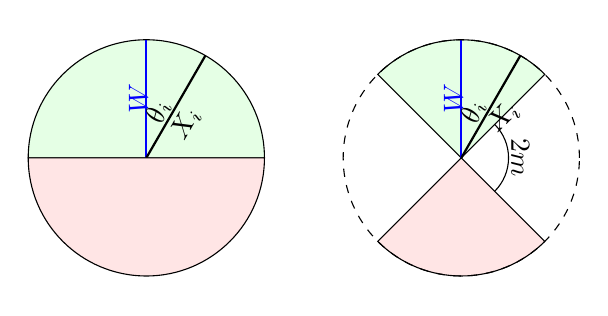
\begin{tikzpicture}
		% the origin
		\def\r{1.5}
		\def\d{2}
		\def\rad{0.707106}
		
		
		%\draw[help lines] (-2,-4) grid (+2,+4);
		
		\draw[fill=green!10] (-\d,0) -- (-\d+\r,0) arc[start angle=0, end angle=180,radius=\r cm] -- (-\d,0);
		
		\draw[thick,blue] (-\d,0) -- (-\d,\r);
		\node[color=blue , rotate=90] at (-\d-0.05*\d,\r/2) {$W$};
		\node[color=black , rotate=60] at (-\d+\r/3,\r * 0.8660/3) {$X_i$};
		%	\draw[color=blue] at (-4,2) {\texttt{$W$}};
		\draw (-\d,\r/3) arc [start angle=90, end angle=60,radius=\r/3 cm] ;
		\node[color=black , rotate=75] at (-\d+\r/3*1.2*0.2588,\r/3*1.2*0.9659) {$\theta_i$};
		%\draw (-4+0.5,0.8660) arc [start angle=60, end angle=90,radius=1 cm] (-4,1);
		\draw[thick,black] (-\d,0) -- (-\d+\r/2,\r * 0.8660);
		\draw[fill=red!10] (-\d,0) -- (-\d-\r,0) arc[start angle=180, end angle=360,radius=\r cm] -- (-\d,0);
		
		\draw[fill=green!10] (\d,0) -- (\d+\r*\rad,\r*\rad) arc[start angle=45, end angle=135,radius=\r cm] -- (\d,0);
		
		\draw[thick,blue] (+\d,0) -- (+\d,\r);
		\node[color=black , rotate=44] at (\d+\r/2*0.7193,0.694*\r/2) {$X_i$};
		\node[color=blue , rotate=90] at (\d-0.05*\d,\r/2) {$W$};
		\draw[thick,black] (\d,0) -- (\d+\r/2,\r * 0.8660);
		\draw[fill=red!10] (\d,0) -- (\d-\r*\rad,-\r*\rad) arc[start angle=225, end angle=315,radius=\r cm] -- (\d,0);
		
		\draw (\d,\r/3) arc [start angle=90, end angle=60,radius=\r/3 cm] ;
		\node[color=black , rotate=75] at (\d+\r/3*1.2*0.2588,\r/3*1.2*0.9659) {$\theta_i$};
		
		\draw (\d+\r/3*1.2,0) arc [start angle=0, end angle=45,radius=\r/3*1.2 cm] ;
		\draw (\d+\r/3*1.2,0) arc [start angle=0, end angle=-45,radius=\r/3*1.2 cm] ;
		\node[color=black , rotate=270] at (\d+\r/2,0) {$2m$};
		\draw[dashed] (\d,0) circle (\r cm);
		%\draw[thick]
		
		
		%\draw[dashed,red] (-3.5,0) circle (3cm) 
		
		%\draw (1,2) coordinate(a) circle (2pt);
	\end{tikzpicture}
	
	\caption{comparing arcb and bce }
	\label{fig:arcb}
\end{figure}

f the cost function is optimized properly, it causes the property vectors in the cosine space to be arranged in the final layer in such a manner that the angle between the new sample and the weight vector approaches zero in the case of label one, and is inclined to in the case of label zero. Additionally, the impact of adding margins on the divisibility of the two classes is readily apparent. On the ideal left, Figure (2-3) illustrates the outcome of separating feature vectors using the BCE cost function. And to the right of the ARCB cost function, a margin in the cosine space is used to divide the feature vectors.

\subsection{PID loss}

There are multiple live examples and several counterfeit samples for each individual in the extant datasets in the area of face anti spoofing. That is, a person's face has been utilized to gather data and a sample of his live and false video has been captured. There is an identical look characteristic in both the genuine and false video of the person in the database, including the parts of his face that are distinct from the other person. On the other hand, it is preferable for the network to concentrate on the indicators of spoof on the face throughout the training phase, rather than on the facial characteristics.
Since the network's primary input picture contains the face and facial characteristics of a person, the network will tend to focus on those aspects for various samples, which is undesirable.
As a result, a penalty is applied to the cost function in this section. In this scenario, the network's objective is to disregard physical traits of people in favor of qualities associated with fraud.
Assume the following is the output property vector of the attribute extraction step for the k-th individual designated l:
$X_k^l \in R^d , I \in \{0,1\}, K \in \{1,2,...,M\}$

This indicates that the database has the sample tag for a number zero or one, as well as the sample tag for a number M of distinct individuals.

Each phase of training assumes the existence of N batch size. There are ${N\choose 2}$ attribute vector pairings among them, of which two states are significant.

The first instance occurs when two attribute vectors in pairs are associated with the same individual but have distinct labels. That is Given that the physical traits of the individual represented by the primary input picture are identical, it is important to maximize the distance between these two samples in this situation. By increasing this distance, the network is compelled to focus on the feature that distinguishes the two cases, rather than on the physical traits of the individuals, which is the difference in the label of these two feature vectors, one real and one fictitious.

This mode is seen in Figure (3-3). In this illustration, the top image is a real one, while the bottom one is a fake. Due to the similarity of these two photos, the output of their feature vectors may be identical. In the following d space, feature vectors are shown as stars. This distance must be increased as much as possible. Thus, in the first scenario, the network serves as a conduit for communication (3.14).

\begin{equation}\label{eq:pid1obj}
	\max_{\Theta} {d( X_{k_1}^{l_1},X_{k_2}^{l_2} )} = \min_{\Theta}{\max(0,M-d( X_{k_1}^{l_1},X_{k_2}^{l_2} ))}
\end{equation}

Where  denotes the set of lattice weights and d is the Euclidean distance between the two property vectors adjusted as Equation (3.15).

  \begin{equation}\label{eq:dfunc}
	d(X_1,X_2) = ||\frac{X_1}{||X_1||}-\frac{X_2}{||X_2||}||
\end{equation}
Because the cost function must be reduced during optimization, increasing the distance between the two feature vectors is equal to decreasing the value
$\max(0,M-d( X_{k_1}^{l_1},X_{k_2}^{l_2} ))$ M is a hyperparameter in this context; if the distance between two attribute vectors is more than this value, the output value is zero; if it is smaller, the distance to this value M is the cost value.
Due to the inequality in Equation (3.16), the greatest distance between two property vectors in normalized space is 2, and hence the cost value of M is two in the implementation of this function.

  \begin{equation}\label{eq:ne}
	||\frac{X_1}{||X_1||}-\frac{X_2}{||X_2||}|| \le ||\frac{X_1}{||X_1||}||+||\frac{X_2}{||X_2||}||   \to d(X_1,X_2) \le 2
\end{equation}

The second instance is when two attribute vectors in pairs have the same label but are associated with distinct individuals. Mathematically, . Due to the physical qualities of the two properties vectors, they may have a substantial distance in the property space in this situation. It is desired to minimize the distance between the two feature vectors in this scenario. In this situation, the network is required to pick the feature image in such a manner that the distance between the two feature vectors is as minimal as possible, and by accomplishing this aim, the extracted features will be more focused on fraud detection characteristics than on physical traits of persons. have.
This circumstance is shown in Figure (3-4). The two input photographs in this example are both fictitious but belong to distinct individuals. The star marks the location of the feature vector corresponding to these two inputs in the subsequent d space in this picture. Due to the fact that two individuals have very distinct physical traits, the distance between their respective property vectors may be quite varied. In this scenario, it is meant to shorten this distance.
Thus, in mathematical words, the cost function in this situation will take the shape of a relation (3.17).
\begin{equation}\label{eq:pid2obj}
	\min_{\Theta} {d( X_{k_1}^{l_1},X_{k_2}^{l_2} )} 
\end{equation}
Finally, the cost function will be dependent on the database's users' IDs as relation (3.18):
\begin{multline}\label{eq:pid}
	L_{PiD} = \sum_{l_1 \ne l_2,k_1 \ne k_2}\frac{1}{N_i}d( X_{k_1}^{l},X_{k_2}^{l}) \\
	+\frac{1}{N_j}\max(0,M-d( X_{k}^{l_1},X_{k}^{l_2} ))
\end{multline}

Where is the number of pairs of samples sharing the same tag attribute but belonging to a different individual in the batch, and   denotes the number of pairs of samples sharing the same tag attribute but sharing the same ID.

The cost function is formed by selecting all pairings that have the same identifier condition of the same label or the same identifier condition-different label from the N sample in each training step and inserting their Euclidean distance in Equation (3.18). When this cost function is reduced, the network is steered toward identifying useful traits for detecting fraud and away from features associated with people's appearance.
Finally, the entire cost of network training will be expressed as a percentage (3.19).

\begin{equation}\label{eq:ltot}
	L_{overal} = \lambda_1L_{ArcB} + \lambda_2L_{PiD}
\end{equation}

Where  and  are hyper parameters indicating the degree of focus placed on each.

\section{implementation details}

The Python programming language and the Pytorch library are used in this article. This library is a very capable modeler of deep networks.
Pytorch's greater versatility compared to other tools makes it simpler to create new functions and unexpected operations.

This paper offers a new LBP operator and a novel cost function that are not readily accessible as modules in deep learning programs but can be implemented using Pytorch computation streams.

To implement a new operator with a learnable argument, a class derived from nn.Module must be written. This will be capable of both forward and reverse computation and can be utilized in deep network computing.

To enable this class to have learning parameters, the class parameter variable must be written using nn.Parameter. If this operator is employed as a layer in a network, the LBP operator parameters will be included in the network parameters, and optimization will result in these parameters being updated.

Each time input is passed to the network after the extraction block, the property of a vector is retrieved, which must be normalized at each step before being used in the two cost functions introduced. One normalization will serve for network testing, since there will be no change in weights. The ARCB function is implemented using Pytorch functions to ensure computational stability. Drop out [36] was employed in the last layer after normalizing the feature vector and before the classifier to avoid over-fitting the data.
To implement the cost function based on the identities of the individuals, in addition to the input picture and image label, an identifier in the form of a number is required. In current datasets, the ID number may be deduced from the video file's name. The network has been optimized using the Adam method [35].

To load and prepare data, the Pythoch library has pre-defined methods and classes that will automatically utilize the photographs in a folder, but owing to the video nature of the data and the unique cost function presented, it is not feasible to use pre-defined functions.

In certain datasets, there is a file for face coordinates that can be extracted from each video frame, the portion connected to the face, and instead of utilizing the whole frame as input to the network to be supplied, just the portion of the face with a little amount of the image's backdrop may be used. In datasets that lack this coordinate file, the faces of the frames are located and recorded in a text file using the MTCCN technique [32].
All of the datasets presented here are in the form of video. Since the suggested technique operates on a single image, one of the more practical aspects of teaching with video data is preparing the data for training. One method is to convert the video to a picture and store it on the hard drive. This, however, will occupy a significant amount of disk space and significantly slow down the training process, since the pictures will need to be reloaded from drive to RAM during training.

On the other hand, since the samples in the two classes are not equal, it is important to have nearly the same amount of films from each class in each category in order to stabilize the ARCB cost function. On the other hand, in order for the cost function based on person IDs to operate effectively, the video must be sufficiently dispersed within each category so that there are distinct examples of individuals with distinct IDs and labels inside each category. Additionally, it is vital for the data to be as random as possible in order to provide additional uncertainty for the network during training.
To implement the approach described in this paper, the video will first be put into RAM in batches, and then a frame will be randomly picked from each video in each batch. Finally, there will be a frame for training in each batch. Had. The next phases will use the same videos that were put into RAM, and this procedure will continue as long as there is a frame in the films. Then another video genre will be chosen, and training will continue on all videos.

Because the number of frames is repeated and the training stages are repeated sequentially after picking a number of films, and the subsequent frames of a video are visually near to one another, it is important that the data has a greater degree of uncertainty. This is accomplished via the use of random data augmentation techniques. To do this, converters are utilized that randomly rotate each input picture.
To avoid over-fitting, the technique of mistakenly removing a portion of the input picture was applied [40]. Additionally, when the face is to be cut off from the backdrop, this is done using a random window; hence, each time the data is loaded, the location of the face in the cropped picture is random and will not always be in the image's center.
Figure (4-1) demonstrates how to cut the face randomly with the backdrop. The blue rectangle represents the person's face in this photograph, while the colorful rectangles are randomly picked for each face selection.

\begin{figure}[ht]
	\centerline{\includegraphics[width=\linewidth]{aug}}
	\caption{random cropping around face}
	\label{fig:aug}
\end{figure}
To create the data loading class, a custom batch sampler was built, as well as a custom batch sampler function to execute the technique of randomly choosing video and reusing successive video frames.
This function is implemented using the Python programming language's iteration notion.

evaluation metrics:

The fraud detection issue is a two-class classification problem that often does not provide an equal number of genuine and counterfeit samples when evaluated.
As a result, the network accuracy criteria, defined as the number of properly predicted samples divided by the total number of samples, is insufficient for evaluating network performance.

This is accomplished by using a criterion known as equal error rate and visualizing it for various thresholds in the form of an equal error rate diagram.

Two modes are critical in constructing this graphic.
Sample acceptance error rate, which indicates that the tag was really a real person but was expected to be a phony person.
Additionally, there is a rejection error rate, which indicates that the sample contains a fictitious label but is projected as a live face.

\begin{equation} \label{eq:far}
	FAR = \frac{number\; of\; false\; accepted\; samples}{total\; number\; of\; fake\; samples}
\end{equation}
\begin{equation} \label{eq:frr}
	FAR = \frac{number\; of\; false\; rejected\; samples}{total\; number\; of\; real\; samples}
\end{equation}

This value is often determined using one of the factors as a threshold. For example, the value of a single layer of neurons in the last layer of a neural network with a sigmoid activation function will be between zero and one. A judgment is made to forecast the sample label by setting a threshold level and comparing the number of neurons in the final layer to this threshold level. The error rate is equal to the figure obtained by multiplying FAR by FRR.

The graph in Figure (4-2) illustrates this criteria at various threshold values.
In datasets with three parts: training, development, and test, the network weights are typically acquired on the training data, whereas the parameter $_EER *$ is obtained on the development data.
Additionally, the standard half of the error rate is specified in the test section as Equation (4.5).


\begin{equation}\label{eq:taueer}
	\tau_{EER} = \argmin_{\tau}|FAR(\tau)-FRR(\tau)|
\end{equation}
\begin{equation}\label{eq:eer}
	EER=FAR(\tau_{EER})=FRR(\tau_{EER})
\end{equation}

\begin{equation}\label{eq:hter}
	HTER=\frac{FAR(\tau_{EER})+FRR(\tau_{EER})}{2}
\end{equation}

We may examine the network's performance by evaluating the equal error rate diagram.
The less the FRR and FAR curves overlap, the more accurate the network.
The FRR and FAR values around the junction also indicate how far apart the two classes are separated by the network.

Another criteria for assessing the usage of ISO / IEC 30107-3 is the definition of attack presentation classification error rate (APCER) and excellent presentation classification error rate (BPCER), the latter of which is similar to the FRR.
However, APCER is comparable to the maximum FAR for many assault instruments.

A printed paper assault or a replay attack are both examples of attack tools.
Additionally, the average categorization error rate is defined as the product of the APCER and BPCER averages.

\begin{equation}\label{eq:apcer}
	APCER=\max_{PAI=1,...,C}{FAR_{PAI}}
\end{equation}
\begin{equation}\label{eq:ACER}
	ACER=\frac{APCER+BPCER}{2}
\end{equation}

\section{experimental results }

This section evaluates the proposed method's accuracy on a variety of datasets. To begin, the proposed approach is evaluated for efficacy on the Replay database, which is a relatively small database.

This is done in order to proof of concept. Following that, accuracy is provided for more datasets. To assess the offered strategies and their influence on accuracy improvement, an ALEXNET network with a BCE cost function is initially employed. Figure illustrates the curve of the equal error rate in this situation (4-3). As can be observed, using the 0.13 threshold level for the last neuron results in an unnoticed error of 7.3 percent. However, it should be noted that not only the magnitude of the error is significant, but also the performance of the graph in other sections of the threshold level, and at 0.6, the FRR error value is almost 80\%, which is very high. Additionally, around the 0.13 threshold level, the error value rises when the threshold level is changed slightly.

\begin{figure}[h]
	\centerline{\includegraphics[width=\linewidth]{eer-alex-bce}}
	\caption{EER}
	\label{fig:eer-alex-bce}
\end{figure}

The diagram in Figure 4-4 is created by training the LBP operator before to ALEXNET with a BCE cost function.

\begin{figure}[h]
	\centerline{\includegraphics[width=\linewidth]{eer-lbp}}
	\caption{eer}
	\label{fig:eer-lbp}
\end{figure}

As can be observed, by employing just one LBP layer before to ALEXNET, the error rate was decreased to 0\%. Additionally, the error status at the threshold has been enhanced.
Given that the inclusion of a layer of trainable LBP operators adds minimal computational complexity to the network, Figure compares the other network training diagram with the BCE cost function and the efficient net B0 network (4-5).

\begin{figure}[h]
	\centerline{\includegraphics[width=\linewidth]{eer-eff}}
	\caption{eer}
	\label{fig:eer-eff}
\end{figure}

This figure demonstrates that using a complicated network does not always result in the intended outcome.
It is important to note that this graphic does not imply that the LBP layer with ALEXNET is more powerful than the Efficient network. Rather than that, in this specific application and replay datasheet, which contains a little quantity of data, utilizing a simpler but smarter network, depending on the problem, results in increased accuracy.

At the moment, just the ALEXNET network without the LBP operator is employed, but the newly released ARCB cost function is used in place of the BCE function.

\begin{figure}[h]
	\centerline{\includegraphics[width=\linewidth]{eer-arcb}}
	\caption{arcb}
	\label{fig:eer-arcb}
\end{figure}

The design in Figure (4-6) demonstrates that it is possible to alter the cost function without altering the structure. The graphic is symmetrical in comparison to the preceding ones. The error rate is zero near the threshold level in this figure, but grows as the distance between the threshold level and the values 0 and 1 increases. This margin impact on the ARCB cost function is what results in the separation of two classes by a margin

\begin{figure}[!h]
	\centerline{\includegraphics[width=\linewidth]{eer-pid}}
	\caption{pid}
	\label{fig:eer-pid}
\end{figure}

The basic ALEXNET structure is now employed, and the classifier's cost function is the BCE function, but a cost function depending on the person's identification has been added as well. This situation is shown graphically in Figure (4-7). As can be observed, the error between the 0 and 0.8 criteria is nil. Which demonstrates that the two classes are sufficiently divided.

Until now, the impact of each suggested approach has been investigated independently. To proceed with the chapter, all approaches are combined. And the extraction network is a characteristic of an Efficient network. Additionally, to aid in the network's convergence, the feature extraction part makes use of weights learned on the image-net database, although these weights vary during the training process.
The picture resolution of the MSU and CASIA datasets is greater than that of the Replay datasets. In contrast to replay datasets, which are divided into three components: training, development, and testing, these datasets are divided into two components: training and testing. The value of the equal error rate is presented in the data test section of Table (4-1).
\begin{table}[!h]
	\caption{casia and msu}
	\label{tab:eercasiamsu}
	\centering
%	\onehalfspacing
	\begin{tabular}{|c|c|}
		\hline Dataset & EER (\%)   \\
		\hline CASIA   & 0.54     \\
		\hline MSU     & 0.0 \\
		\hline
	\end{tabular} 
\end{table}

Given the age of these two datasets, it is not difficult to achieve zero precision. Recent research in this area has focused on accuracy using the SIW and OULU datasets. These two datasets are more recent and greater in size than the preceding two. As a result, the majority of these two datasets have been included into contemporary studies. Each of these two datasets has a unique technique that demonstrates distinct methods for assessing the model's generalization.

The first protocol analyses changes in face state using the SIW database. For training purposes, just the first 60 frames of each video are utilized; however, for testing purposes, all frames from the test movies are used. Because the user does not move his face during the first 60 seconds of each video, the training data comprises only photos of the face in a fixed location in front of the camera. However, the test data covers all of the video's face movement phases. This protocol demonstrates the proposed model's generalization across many face modalities. The outcome of this instance is summarized in Table (4-2) along with a comparison to many well-known methodologies.

\begin{table}[h]
	\caption{siw 1}
	\label{tab:siw1}
	\centering
%	\onehalfspacing
	\begin{tabular}{|c|c|c|l|}
		\hline ACER & BPCER & APCER & Method                \\
		\hline 3.58 & 3.58  & 3.58  & \cite{liu2018learning} Auxiliary    \\
		\hline 0.25 & 0.50  & 0     & \cite{feng2020learning} LGSC         \\
		\hline 1    & -     & -     & \cite{yang2019face} STASN       \\
		\hline 0.12 & 0.17  & 0.07  & \cite{yu2020searching} CDCN             \\
		\hline 0.4  & 0.17  & 0.64  & \cite{wang2020deep} SGTD      \\
		\hline 0.4  & 0.17  & 0.69  & \cite{li20203dpc}   3DPC-NET   \\
		\hline 0.13 & 0.12  & 0.14  & ARCB+PID    \\ 
		\hline         
	\end{tabular}
\end{table}

In the second protocol, one of the four kinds of replay assaults is reserved for testing each time, while the other three are used for network training. Thus, this technique has four distinct modes in which the mean and variance accuracy are presented. This protocol is intended to evaluate the suggested method's performance against an unobserved replay assault. The findings are summarized in Table (4-3).

\begin{table}[!h]
	\caption{siw 2 }
	\label{tab:siw2}
	\centering
	%	\onehalfspacing
	\begin{tabular}{|c|c|c|l|}
	\hline ACER      & BPCER   & APCER     & Method              \\
	\hline 0.57 ±0.69& 0.57 ±0.69  & 0.57 ±0.69& \cite{liu2018learning} Auxiliary \\
	\hline 0±0       & 0±0     & 0±0       & \cite{feng2020learning} LGSC       \\
	\hline 0.28±0.05 & -           & -             & \cite{yang2019face} STASN       \\
	\hline 0.04±0.5  & 0±0.09  & 0±0       & \cite{yu2020searching} CDCN        \\
	\hline 0.02±0.04 & 0.04±0.08   & 0.0±0.0   & \cite{wang2020deep} SGTD    \\
	\hline 0.45±0.14 & 0.43±0.06   & 0.46±0.28 & \cite{li20203dpc}   3DPC-NET   \\
	\hline 0.0087±0.0151 & 0.01±0.0173 & 0.0075±0.0129 & ARCB+PID            \\
	\hline         
\end{tabular}
\end{table}

Additionally, the OULU database contains four distinct protocols, the correctness of which is demonstrated in this paper's first and second protocols.
Three separate sites have been used to photograph the OULU database. The first protocol involves training on films linked to the first and second positions, while the second protocol involves doing the test on movies connected to the third place. This protocol is being offered with the intent of analyzing the suggested method's capabilities by shifting the images.

The second protocol stores two printed paper attacks and two replay attacks in the database; one print attack and one replay attack are used for training, while the other print and replay attack is used for testing. The goal of this procedure is to assess instruments that are not often encountered during training. The first and second procedures report on the correctness of the model described in Table (4-4).

\begin{table}[h]
	\caption{oulu1 }
	\label{tab:oulu1}
	\centering
%	\onehalfspacing	
\begin{tabular}{|c|c|c|l|}
		\hline               
		ACER & BPCER      & APCER & Method              \\
	\hline 5.7     & 8.9        & 2.5 & \cite{tu2020learning}GFA     \\
	\hline 1.6     & 1.6        & 1.6  & \cite{liu2018learning} Auxiliary     \\
	\hline 1.5     & 1.7        & 1.2  & \cite{jourabloo2018face} FaceDs\\
	\hline 0.4     & 0          & 0.8  & \cite{feng2020learning} LGSC   \\
	\hline 1.9     & 2.5        & 1.2 & \cite{yang2019face} STASN   \\
	\hline 0.2     & 0          & 0.4  & \cite{yu2020searching} CDCN   \\
	\hline 1.0     & 0.0        & 2.0  & \cite{wang2020deep} SGTD   \\
	\hline 0.42 & 0          & 0.83& \cite{george2019deep} {DeepPixBis}\\
	\hline 1.1     & 1.3        & 0.8  & \cite{liu2020disentangling}STDN \\
	\hline 1.2     & 0          & 2.3 & \cite{li20203dpc}      3DPC-NET      \\
	\hline 2.29 & 2          & 2.58& ARCB+PID \\              
\hline         
\end{tabular}
\end{table}

\begin{table}[ht]
	\caption{oulu2}
	\label{tab:oulu2}
	\centering
%	\onehalfspacing
	\begin{tabular}{|c|c|c|l|}
		\hline             
		ACER &      BPCER          &      APCER &      Method                  \\
		\hline          1.9        &      1.3        &      2.5        & \cite{tu2020learning}     GFA  \\
		\hline          2.7        &      2.7        &      2.7        & \cite{liu2018learning}      Auxiliary  \\
		\hline         4.3        &      4.4        &      4.2        & \cite{jourabloo2018face}      FaceDs    \\
		\hline        0.7        &      0.6        &      0.8        & \cite{feng2020learning}      LGSC       \\
		\hline          2.2        &      0.3        &      4.2        & \cite{yang2019face}      STASN       \\
		\hline         1.3        &      0.8        &      1.8        & \cite{yu2020searching}      CDCN       \\
		\hline       1.9        &      1.3        &      2.5        & \cite{wang2020deep}      SGTD       \\
		\hline      6.0        &      0.6        &      11.4        & \cite{george2019deep}      DeepPixBis\\
		\hline      1.9        &      1.6        &      2.3        & \cite{liu2020disentangling}     STDN     \\
		\hline       3.0        &      2.8        &      3.1        & \cite{li20203dpc}        3DPC-NET        \\
		\hline       0.97 &      0.97           &      0.97        &      ARCB+PID \\              
		\hline         
	\end{tabular}
\end{table}





\subsection{corss dataset test}
As seen in the preceding sections, achieving an error rate close to zero is not out of reach using new deep learning algorithms. However, how the suggested model performs on unknown data with varying distributions remains a difficult and critical subject in academic study. While a model may achieve great accuracy on a data set with a certain distribution, it performs badly in the actual world.

Thus far, the findings have shown the model's accuracy inside the database. Another critical challenge in the realm of fraud detection is the reproducibility of tests performed on two distinct datasets. This is accomplished by training the model on one dataset and testing it on another.

To validate the model's accuracy while comparing datasets, the network is trained on the CASIA dataset and then evaluated on the Replay dataset. Table (4-5) summarizes the outcome of this case, as well as the accuracy of previous investigations.

\begin{table}[!h]
	\caption{cross test resulat }
	\label{tab:cross}
	\centering
%	\onehalfspacing
\begin{tabular}{|c|l|}
\hline HTER \% & Method             \\
\hline 31.5        & \cite{yang2019face} STASN \\
\hline 17          &  \cite{wang2020deep} SGTD \\
\hline 27.6        & \cite{liu2018learning} Auxiliary   \\
\hline 28.5        & \cite{jourabloo2018face} FaceDs\\
\hline 21.4        & \cite{tu2020learning}GFA  \\
\hline 27.4        & \cite{feng2020learning} LGSC \\
\hline 23.4        & \cite{li20203dpc}   3DPC-NET \\
\hline 21.25        & ARCB+PID \\ 
\hline
\end{tabular}
\end{table}
\subsection{computational cost }

a metric for measuring the neural network's speed of execution
A computer's ability to do floating point operations

Afterwards, when the network has been completed.
This value is expressed in (Mac.) units.
FLOPs (whatever the value)

The smaller the network, the cheaper the computing cost, and hence the faster the network will be.
Comparison of the computing costs of the approaches that were proven accurate in the preceding section is shown in Table 7.4.

The proposed approach of this dissertation is also described, along with the computing costs.

From this table, it is clear that the proposed method's computing costs are a long way off.

Other procedures are employed.
EfficientNet B0 is the network's primary processing mechanism.

Comparatively speaking, the network's computing costs will be substantially lower.
There is no need to have a large amount of computing power in order to use this strategy.

While minimizing processing costs, it should be emphasized that the suggested method's accuracy is in many circumstances superior to other approaches and in some cases Accurately competitive with current methods.

Unlike [10] CDCN, [8] Auxiliary and [43] SGTD methods and STASN, [8] Auxiliary methods, the proposed method did not use depth as an auxiliary signal.
There are no video sequences required for the evaluation of SGTD, and it functions as a single frame. 


\begin{table}[!h]
	\caption{flops compariation }
	\label{tab:flops}
	\centering
%	\onehalfspacing
	\begin{tabular}{|c|l|}
		\hline FLOPs					& Method  \\
		\hline 50.9 GMac		 		& \cite{liu2018learning} Auxiliary   \\
		\hline 47.48 GMac 				&\cite{yu2020searching} CDCN \\
		\hline 39.4 GMac 				&\cite{liu2020disentangling} STDN \\
		\hline 4.64 GMac 				& \cite{george2019deep} DeepPixBis \\
		\hline 9.53 GMac 				&\cite{feng2020learning} LGSC        \\
		\hline 15.38 GMac 				&\cite{tu2020learning} GFA	\\
		\hline 1.82 GMac 				& \cite{li20203dpc}   3DPC-NET \\	
		\hline 400.39 MMac 				& ARCB+PID \\
		\hline
	\end{tabular}
\end{table}




% You must have at least 2 lines in the paragraph with the drop letter
% (should never be an issue)


%\hfill mds
 
%\hfill August 26, 2015

%\subsection{Subsection Heading Here}
%Subsection text here.

% needed in second column of first page if using \IEEEpubid
%\IEEEpubidadjcol

%\subsubsection{Subsubsection Heading Here}
%Subsubsection text here.


% An example of a floating figure using the graphicx package.
% Note that \label must occur AFTER (or within) \caption.
% For figures, \caption should occur after the \includegraphics.
% Note that IEEEtran v1.7 and later has special internal code that
% is designed to preserve the operation of \label within \caption
% even when the captionsoff option is in effect. However, because
% of issues like this, it may be the safest practice to put all your
% \label just after \caption rather than within \caption{}.
%
% Reminder: the "draftcls" or "draftclsnofoot", not "draft", class
% option should be used if it is desired that the figures are to be
% displayed while in draft mode.
%
%\begin{figure}[!t]
%\centering
%\includegraphics[width=2.5in]{myfigure}
% where an .eps filename suffix will be assumed under latex, 
% and a .pdf suffix will be assumed for pdflatex; or what has been declared
% via \DeclareGraphicsExtensions.
%\caption{Simulation results for the network.}
%\label{fig_sim}
%\end{figure}

% Note that the IEEE typically puts floats only at the top, even when this
% results in a large percentage of a column being occupied by floats.


% An example of a double column floating figure using two subfigures.
% (The subfig.sty package must be loaded for this to work.)
% The subfigure \label commands are set within each subfloat command,
% and the \label for the overall figure must come after \caption.
% \hfil is used as a separator to get equal spacing.
% Watch out that the combined width of all the subfigures on a 
% line do not exceed the text width or a line break will occur.
%
%\begin{figure*}[!t]
%\centering
%\subfloat[Case I]{\includegraphics[width=2.5in]{box}%
%\label{fig_first_case}}
%\hfil
%\subfloat[Case II]{\includegraphics[width=2.5in]{box}%
%\label{fig_second_case}}
%\caption{Simulation results for the network.}
%\label{fig_sim}
%\end{figure*}
%
% Note that often IEEE papers with subfigures do not employ subfigure
% captions (using the optional argument to \subfloat[]), but instead will
% reference/describe all of them (a), (b), etc., within the main caption.
% Be aware that for subfig.sty to generate the (a), (b), etc., subfigure
% labels, the optional argument to \subfloat must be present. If a
% subcaption is not desired, just leave its contents blank,
% e.g., \subfloat[].


% An example of a floating table. Note that, for IEEE style tables, the
% \caption command should come BEFORE the table and, given that table
% captions serve much like titles, are usually capitalized except for words
% such as a, an, and, as, at, but, by, for, in, nor, of, on, or, the, to
% and up, which are usually not capitalized unless they are the first or
% last word of the caption. Table text will default to \footnotesize as
% the IEEE normally uses this smaller font for tables.
% The \label must come after \caption as always.
%
%\begin{table}[!t]
%% increase table row spacing, adjust to taste
%\renewcommand{\arraystretch}{1.3}
% if using array.sty, it might be a good idea to tweak the value of
% \extrarowheight as needed to properly center the text within the cells
%\caption{An Example of a Table}
%\label{table_example}
%\centering
%% Some packages, such as MDW tools, offer better commands for making tables
%% than the plain LaTeX2e tabular which is used here.
%\begin{tabular}{|c||c|}
%\hline
%One & Two\\
%\hline
%Three & Four\\
%\hline
%\end{tabular}
%\end{table}


% Note that the IEEE does not put floats in the very first column
% - or typically anywhere on the first page for that matter. Also,
% in-text middle ("here") positioning is typically not used, but it
% is allowed and encouraged for Computer Society conferences (but
% not Computer Society journals). Most IEEE journals/conferences use
% top floats exclusively. 
% Note that, LaTeX2e, unlike IEEE journals/conferences, places
% footnotes above bottom floats. This can be corrected via the
% \fnbelowfloat command of the stfloats package.




\section{Conclusion}
The current state of the art in the area of face authentication system security was studied in this paper. Historically, techniques have relied heavily on auxiliary cues such as depth. Consecutive video frames have also been employed in a variety of ways to determine if a face is genuine or not. This paper develops a system based on the use of a single frame. Additionally, the suggested solution eliminates the necessity for a depth signal as an auxiliary signal. However, the suggested technique in the first and second protocols achieved comparable accuracy to existing methods in both big and fresh datasets in this sector.
Due to the fact that the suggested approach's primary processing is based on an efficient net network, the computational volume of the proposed technique is minimal. It has a quick reaction time owing to the utilization of a frame.
This paper presents a novel CNN-scalable LBP-based operator. Additionally, when the cost function with margin evolved, the network resolution grew. Additionally, the implementation of a cost function based on the individual's ID improved the network's generalizability. The benefit of utilizing the cost function is that it increases accuracy without increasing the network's computing burden. Thus, although the suggested solution takes extra training time, the network test duration remains constant.
In this study, an efficient net was utilized. Subsequent study may include the usage of buildings that were initially created. Additionally, it might be beneficial to improve the accuracy of the network's attention structure. Increasing accuracy using a new structure may be accomplished by using a video sequence rather of a frame. To improve texture analysis, the LBP amplifier may be enlarged to fit in all levels of the network rather to only its cannula. Instead of a neuron, write. The cost function that is dependent on the person ID may be replaced by other features such as the attack tool. Additionally, employing depth in conjunction with the suggested approach may improve accuracy.
The emphasis of this work is on print and replay assaults. This category contains datasets that involve mask assaults. Further study might be conducted by using a technique similar to the suggested approach to datasets that include RGB and IR pictures.





% if have a single appendix:
%\appendix[Proof of the Zonklar Equations]
% or
%\appendix  % for no appendix heading
% do not use \section anymore after \appendix, only \section*
% is possibly needed

% use appendices with more than one appendix
% then use \section to start each appendix
% you must declare a \section before using any
% \subsection or using \label (\appendices by itself
% starts a section numbered zero.)
%


\appendices
\section{Proof of the First Zonklar Equation}
Appendix one text goes here.

% you can choose not to have a title for an appendix
% if you want by leaving the argument blank
\section{}
Appendix two text goes here.


% use section* for acknowledgment
\section*{Acknowledgment}


The authors would like to thank...


% Can use something like this to put references on a page
% by themselves when using endfloat and the captionsoff option.
\ifCLASSOPTIONcaptionsoff
  \newpage
\fi


\newpage
% trigger a \newpage just before the given reference
% number - used to balance the columns on the last page
% adjust value as needed - may need to be readjusted if
% the document is modified later
%\IEEEtriggeratref{8}
% The "triggered" command can be changed if desired:
%\IEEEtriggercmd{\enlargethispage{-5in}}

% references section

% can use a bibliography generated by BibTeX as a .bbl file
% BibTeX documentation can be easily obtained at:
% http://mirror.ctan.org/biblio/bibtex/contrib/doc/
% The IEEEtran BibTeX style support page is at:
% http://www.michaelshell.org/tex/ieeetran/bibtex/
%\bibliographystyle{IEEEtran}
% argument is your BibTeX string definitions and bibliography database(s)
\bibliographystyle{IEEEtran}
\bibliography{IEEEabrv,MyReferences.bib}
%
% <OR> manually copy in the resultant .bbl file
% set second argument of \begin to the number of references
% (used to reserve space for the reference number labels box)
%\begin{thebibliography}{1}

%\bibitem{IEEEhowto:kopka}
%H.~Kopka and P.~W. Daly, \emph{A Guide to \LaTeX}, 3rd~ed.\hskip 1em plus
%  0.5em minus 0.4em\relax Harlow, England: Addison-Wesley, 1999.

%\end{thebibliography}

% biography section
% 
% If you have an EPS/PDF photo (graphicx package needed) extra braces are
% needed around the contents of the optional argument to biography to prevent
% the LaTeX parser from getting confused when it sees the complicated
% \includegraphics command within an optional argument. (You could create
% your own custom macro containing the \includegraphics command to make things
% simpler here.)
%\begin{IEEEbiography}[{\includegraphics[width=1in,height=1.25in,clip,keepaspectratio]{mshell}}]{Michael Shell}
% or if you just want to reserve a space for a photo:

\begin{IEEEbiography}{Michael Shell}
Biography text here.
\end{IEEEbiography}

% if you will not have a photo at all:
\begin{IEEEbiographynophoto}{John Doe}
Biography text here.
\end{IEEEbiographynophoto}

% insert where needed to balance the two columns on the last page with
% biographies
%\newpage

\begin{IEEEbiographynophoto}{Jane Doe}
Biography text here.
\end{IEEEbiographynophoto}

% You can push biographies down or up by placing
% a \vfill before or after them. The appropriate
% use of \vfill depends on what kind of text is
% on the last page and whether or not the columns
% are being equalized.

%\vfill

% Can be used to pull up biographies so that the bottom of the last one
% is flush with the other column.
%\enlargethispage{-5in}



% that's all folks
\end{document}


